\subsection{Graphene and hydrogen honeycomb lattice (NE-AIDMD)}
Graphene has drawn much attention in the last decade because of its unusual electronic and structural properties and its potential applications in electronics~\cite{Wallace1947, Novoselov2004,NovoselovNature2005, Katsnelson2006, Geim2007, Novoselov2007, neto2009, Castro2009}. 
Although many electronic properties of graphene can be correctly described in a noninteracting electron picture~\cite{Castro2009}, electron-electron interactions do play a central role in a wide range of phenomena that have been observed in experiments~\cite{Kotov2012}. It is also shown that the electron screening from $\sigma$ bonding is very crucial to the correlated physics of graphene, without which graphene would be an insulator instead of a semi-metal \cite{Zheng2016} .

In this section, we will use our downfolding technique to understand the electron correlations of graphene, especially, on how the $\sigma$ electrons affect the overall low energy physics. For comparison, we here also study the hydrogen honeycomb lattice with the same lattice constant $a=2.46$\AA, which has similar Dirac cone dispersion as graphene \cite{Zheng2016}.  We will consider the effective single-band Hubbard model, 
\begin{eqnarray}\label{eq:hubbard}
\hat{H} = C + t\sum_{\langle i,j\rangle}c_{i, \sigma}^\dagger c_{j, \sigma} + \text{h.c.} + U\sum_{i}n_{i, \uparrow}n_{i, \downarrow}\,. 
\end{eqnarray}
The low energy physics is reflected mainly on the dynamics of $\pi$ orbitals in  graphene, and $s$ orbitals in hydrogen. Naturally, we would choose c$_i$ to be the $\pi$ (or $s$) orbitals shown in Fig.~\ref{fig:wan}. Due to lack of screening because of zero density of states at Fermi level, the Coulomb interaction is still long range unlike the case in metal where the Coulomb interaction is short ranged because of the formation of electron-hole pairs. However, the effect of the long range part can be considered as a renormalization to the onsite Coulomb interaction $U$ at low energy \cite{Schuler2013, Changlani2015}. Therefore, we expect that Eq.~\eqref{eq:hubbard} is still a relatively good description of the low energy physics. 

\begin{figure*}[hbt]
  \centering  
 % \subfigure[]{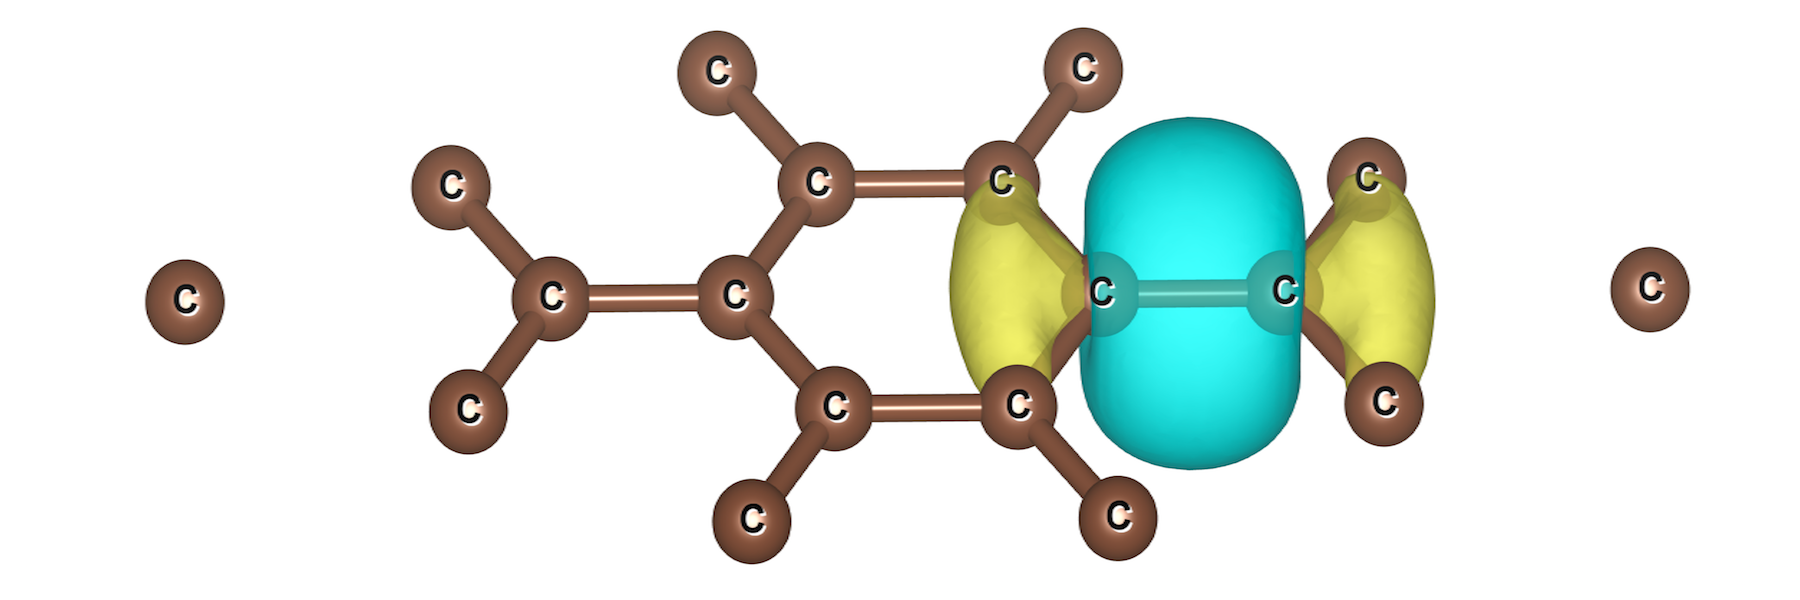
\includegraphics[clip, width=0.30\textwidth]{c_sigma.png}}
    \subfigure[]{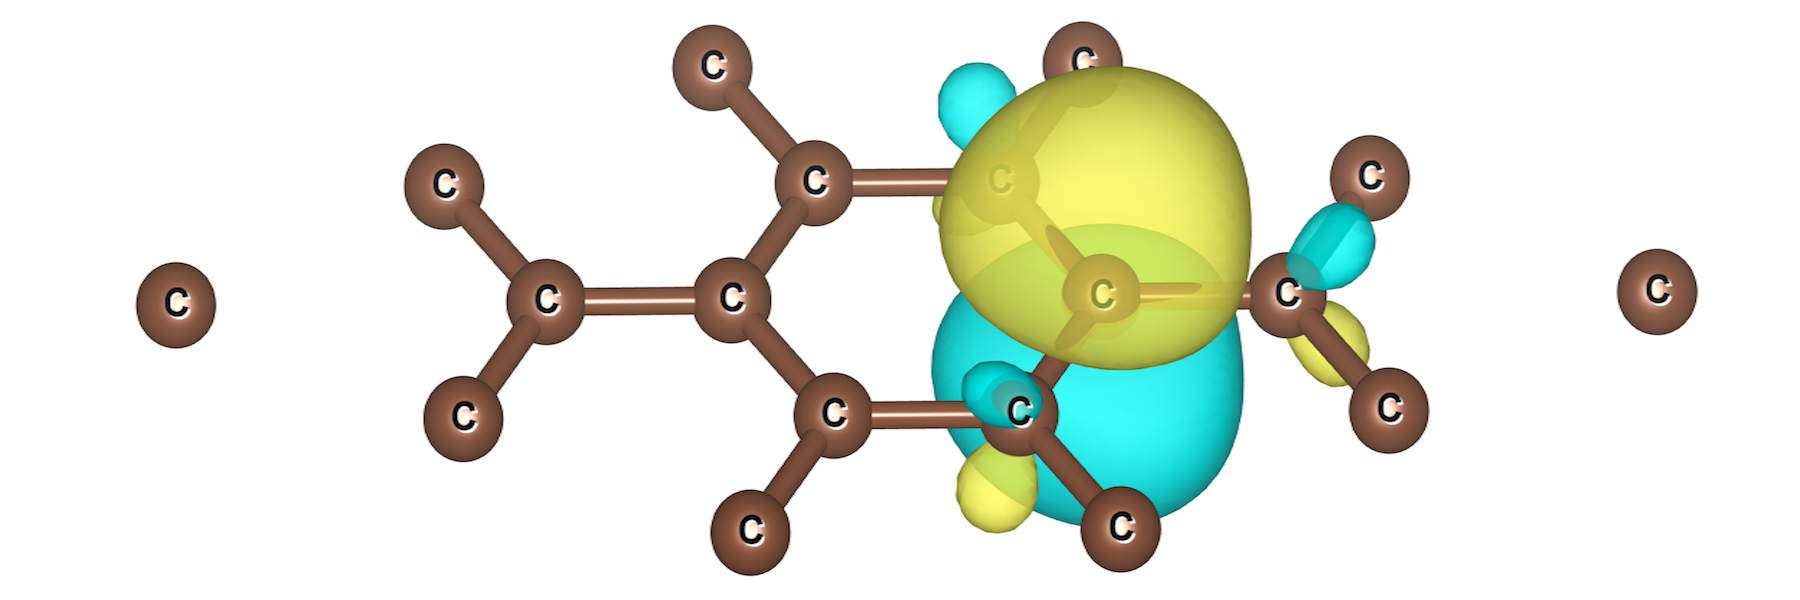
\includegraphics[clip, width=0.30\textwidth]{./Figures/c_pi.png}}
    \subfigure[]{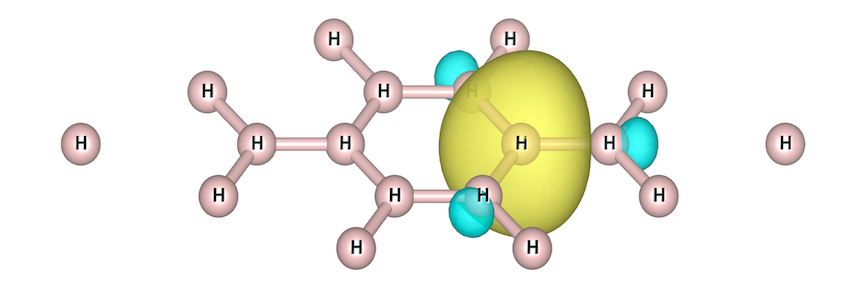
\includegraphics[clip, width=0.30\textwidth]{./Figures/h_wan.png}}
       \caption{Wannier orbitals constructed from Kohn-Sham orbitals: (a) graphene $\pi$ orbitals; (b) hydrogen S orbital. }
\label{fig:wan}
\end{figure*}

We will use the non-eigenstate AIDMD method to obtain the value of $t$ and $U$. In this way, we do not need to solve the model Hamiltonian which is relatively difficult. We choose a set of Slater-Jastrow wave functions corresponding to the electron-hole excitations within the $\pi$ channel (or $s$ channel for hydrogen system). The energy expectation expressed in terms of the density matrices is, 
\begin{eqnarray}\label{eq:en}
E = C + t\sum_{\langle i, j\rangle, \sigma}( \rho_{ij}^\sigma + \rho_{ji}^\sigma) + U \sum_{i}M_{ii;ii}^{\uparrow,\downarrow}\,.
\end{eqnarray}

In order to understand the screening effect of $\sigma$ electrons, we also consider a $\pi$-only graphene, where we replace the $\sigma$ electrons with constant negative charge background. The lower energy states we choose for such systems are Slater-Jastrow wave functions constructed from occupied $\pi$ Kohn-Sham orbitals; whereas for the original graphene, the wave functions are Slater-Jastrow constructed from both occupied $\sigma$ bands and occupied $\pi$ bands. 

Table~\ref{tab:grpheffm} shows the final downfolding results of the three systems. The ab initio simulations are performed on a $3\times3$ cell. We have used using 25 low energy states for the downfolding. The error-bar is calculated using Jackniff method. 

\begin{table}[ht]
\label{tab:grpheffm}
\centering
\begin{tabular}{|c|c|c|c|}
\hline
parameters [eV] & graphene & $\pi$-only graphene &hydrogen \\
\hline
\hline
t & 3.61(1) & 2.99 & 3.73(1)\\
U & 7.16(3) & 14.8(2) & 9.47(5)\\
\hline
\end{tabular}
\caption{Downfolding parameters for graphene and hydrogen.}
\end{table} 
Fig.~\ref{fig:ne_aidmd_gh} shows fitted energies versus the \textit{ab initio} VMC energies. 

We find that the onsite Hubbard model describes graphene and hydrogen very well. The root mean square error of the predicted energies are relatively small (see Fig.~\ref{fig:ne_aidmd_gh}). The ratio of $U/t$ is small than the semi-metal-insulator transition critical value (3.8) in both graphene and hydrogen, which is consistent to the fact that both the two systems are semi-metals.  The $\pi$-only graphene however has larger $U/t$, and is in the insulating phase. This clearly shows the significance of $\sigma$ electrons in renormalizing the effective onsite interactions of $\pi$ orbitals. Without such screening effect, graphene will be an insulator. This is why many previous studies incorrectly predicted graphene to be an insulator in vacuum because they consider only $\pi$ electrons with bare Coulomb interaction \cite{DrutPRL2009, DrutPRB2009,  Smith2014}.

\begin{figure*}[htb]
\centering
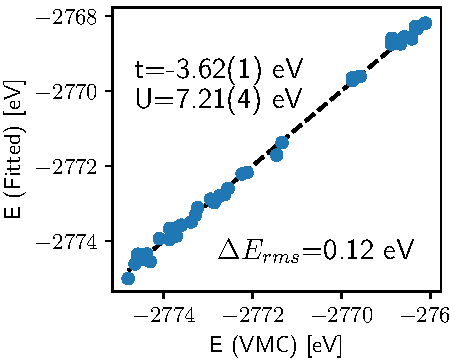
\includegraphics[width=0.32\textwidth]{./Figures/grp_all_tu.pdf}
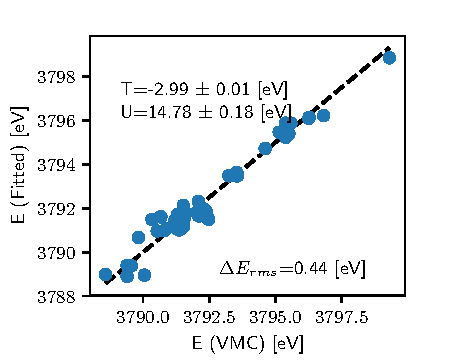
\includegraphics[width=0.32\textwidth]{./Figures/grp_pi_tu.pdf}
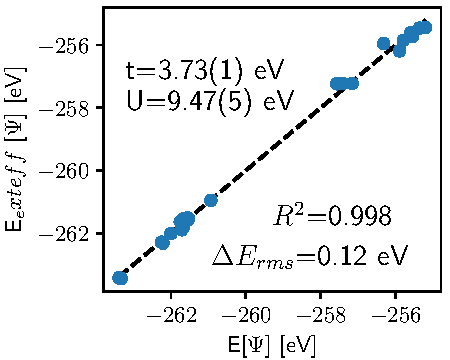
\includegraphics[width=0.32\textwidth]{./Figures/h_tu.pdf}
\caption{Comparison of \textit{ab initio} (x-axis) and fitted energies (y-axis) of the 3$\times$3 periodic unit cell of graphene and hydrogen lattice: (a) graphene; (b) hydrogen lattice.}\label{fig:ne_aidmd_gh}
\end{figure*}

